
% =====================================================================
%  Digital Twin for EV Charging Stations  --  Group 08 project report
%  Compile:  pdflatex report.tex (run twice)   or   tectonic report.tex
%  Figures:  python report/make_figures.py  (from the repository root)
% =====================================================================
\documentclass[11pt,a4paper]{article}

\usepackage{iftex}
\ifPDFTeX
  \usepackage[T1]{fontenc}
  \usepackage[utf8]{inputenc}
  \usepackage{lmodern}
\else
  \usepackage{fontspec}
\fi
\usepackage[a4paper,left=1.7cm,right=1.7cm,top=1.8cm,bottom=1.8cm,headsep=0.4cm]{geometry}
\usepackage{graphicx}
\usepackage{booktabs}
\usepackage{tabularx}
\usepackage{array}
\usepackage{amsmath}
\usepackage{xcolor}
\usepackage[shortlabels]{enumitem}
\usepackage{caption}
\usepackage{fancyhdr}
\usepackage{titlesec}
\usepackage{microtype}
\usepackage[hidelinks]{hyperref}

\definecolor{accent}{HTML}{1F4E79}
\graphicspath{{figures/}}

% ---------- compact, professional layout ----------
\titleformat{\section}{\large\bfseries\color{accent}}{\thesection.}{0.5em}{}
\titleformat{\subsection}{\normalsize\bfseries}{\thesubsection}{0.5em}{}
\titlespacing*{\section}{0pt}{7pt plus 2pt minus 1pt}{3pt plus 1pt}
\titlespacing*{\subsection}{0pt}{5pt plus 1pt minus 1pt}{2pt}
\captionsetup{font=small,labelfont={bf,color=accent},skip=3pt}
\setlength{\parindent}{0pt}
\setlength{\parskip}{3pt plus 1pt}
\setlist{nosep,leftmargin=1.3em}
\setlength{\textfloatsep}{8pt plus 2pt minus 2pt}
\setlength{\floatsep}{6pt plus 2pt minus 2pt}
\setlength{\abovedisplayskip}{3pt}
\setlength{\belowdisplayskip}{3pt}
\renewcommand{\arraystretch}{1.12}

\setlength{\headheight}{14pt}
\pagestyle{fancy}
\fancyhf{}
\fancyhead[L]{\small\color{accent}Digital Twin for EV Charging Stations}
\fancyhead[R]{\small\color{accent}Group 08}
\fancyfoot[C]{\small\thepage}
\renewcommand{\headrulewidth}{0.4pt}

\newcommand{\degC}{\ensuremath{^\circ}C}
\newcommand{\Rsq}{\ensuremath{R^2}}
\newcolumntype{Y}{>{\raggedright\arraybackslash}X}
\newcolumntype{L}[1]{>{\raggedright\arraybackslash}p{#1}}

\begin{document}

% =====================================================================
\begin{center}
  {\LARGE\bfseries\color{accent} Digital Twin for EV Charging Stations}\\[3pt]
  {\large Group 08}\\[2pt]
  \rule{0.6\textwidth}{0.4pt}
\end{center}
\vspace{-4pt}

% =====================================================================
\section{Project Title}
\textbf{Digital Twin for EV Charging Stations.} We built a working digital twin (DT) of a four-bay electric-vehicle
(EV) charging station. Before a car is plugged in, the twin predicts how long the charge will take, how much grid
energy it needs, what it will cost and how much it wears the battery (wear factor, state of health (SOH), remaining
useful life (RUL)), for the station's \emph{current} conditions read from a live temperature sensor.
\begin{itemize}
  \item \textbf{Physical entity:} the charging station and its surroundings; a real LM35 sensor on an Arduino UNO R4
        WiFi measures the ambient temperature at the chargers.
  \item \textbf{Virtual entity:} the station state (bays, sessions, sensor readings, alerts) in MongoDB, a physics
        model of charging, machine-learning (ML) models trained on real public data, and a 3D model of the station.
  \item \textbf{Connection:} sensor data flows into the twin automatically every 5\,s over OPC~UA and MQTT; the twin
        returns predictions, alerts and an animated 3D view to the operator. It advises only and never switches a
        real charger.
\end{itemize}

% =====================================================================
\section{Group Details}
\textbf{Group number:} 08 \qquad \textbf{Project title:} Digital Twin for EV Charging Stations
\begin{center}
\small
\begin{tabular}{@{}cll@{}}
  \toprule
  \textbf{S.\ No.} & \textbf{Name} & \textbf{Roll number} \\
  \midrule
  1 & A.\ Palvash Kumar         & S20230010029 \\
  2 & C.\ Prudhvi Natha Reddy   & S20230010056 \\
  3 & M.\ Narendar              & S20230010149 \\
  \bottomrule
\end{tabular}
\end{center}

% =====================================================================
\section{Block Diagram}
The system runs on three laptops on one LAN (Fig.~\ref{fig:block}): the \emph{sensor laptop} reads the physical
sensor, the \emph{ML laptop} hosts the broker and the models, and the \emph{web laptop} holds the twin's state and UI.

\begin{figure}[!ht]
  \centering
  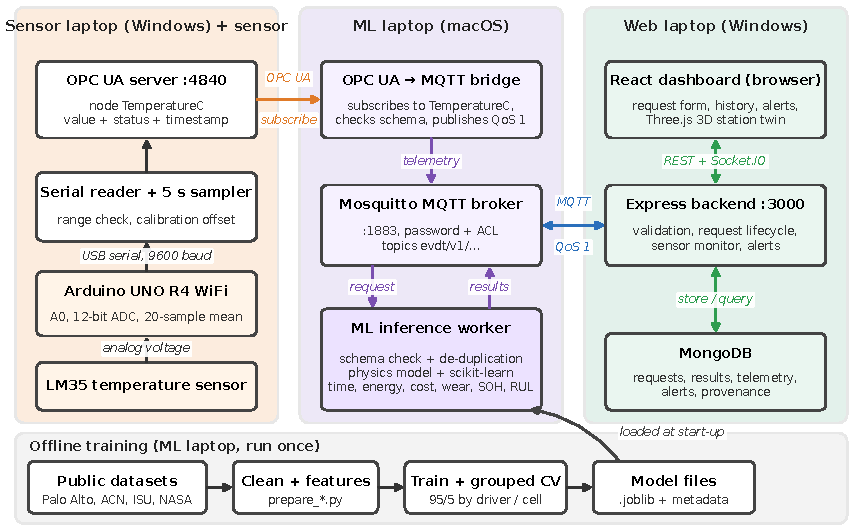
\includegraphics[width=\textwidth]{block_diagram.pdf}
  \caption{Architecture of the digital twin. Coloured arrows are network links between machines. The bottom band
  is the offline training pipeline that produces the model files loaded by the inference worker.}
  \label{fig:block}
\end{figure}

\begin{table}[!ht]
\centering\footnotesize
\caption{How the components communicate.}
\label{tab:links}
\begin{tabularx}{\textwidth}{@{}L{3.9cm}L{3.0cm}YL{1.8cm}@{}}
  \toprule
  \textbf{Link} & \textbf{Protocol} & \textbf{What is sent} & \textbf{Rate} \\
  \midrule
  LM35 $\rightarrow$ Arduino & analog, 12-bit ADC & sensor voltage, averaged over 20 samples & $\approx$2.2\,s \\
  Arduino $\rightarrow$ sensor laptop & USB serial, 9600 baud & text line \texttt{Temperature: 31.26 C}; values outside
      $-50\ldots85$\degC{} rejected & $\approx$2.2\,s \\
  Sensor laptop $\rightarrow$ ML laptop & OPC UA, port 4840 & node \texttt{TemperatureC}: value, status code, source
      timestamp; \emph{Bad} status after 30\,s without data & every 5\,s \\
  Bridge $\rightarrow$ broker & MQTT, QoS 1 & \texttt{evdt/v1/telemetry/temperature} (JSON Schema checked) & every 5\,s \\
  Backend $\leftrightarrow$ ML worker & MQTT, QoS 1 & \texttt{requests/charging}, \texttt{results/charging},
      \texttt{results/health} & per request \\
  Backend $\leftrightarrow$ browser & REST + Socket.IO & requests, results, live station state, alerts & push \\
  Backend $\leftrightarrow$ MongoDB & MongoDB driver & requests, results, telemetry, alerts, provenance & per event \\
  \bottomrule
\end{tabularx}
\end{table}

The broker has one account per component and an access-control list (e.g.\ the bridge may publish only telemetry).
Each message carries a \texttt{messageId} and \texttt{requestId}, so QoS~1 duplicates are dropped and retries are safe.

% =====================================================================
\section{Models}
\subsection{Digital twin model}
The twin keeps a \textbf{state model} of the station: four bays (two Level~2 at 11\,kW, DC fast at 50\,kW and
150\,kW), each with a status (\emph{available}, \emph{charging}, \emph{fault}, \emph{offline}), the active session, the
latest sensor reading with its quality (\emph{live}, \emph{stale}, \emph{suspect}) and open alerts. Every stored value
records its source: \emph{sensor}, \emph{ML estimate}, \emph{physics estimate}, \emph{simulation} or \emph{manual}.

A \textbf{physics model} of charging is the backbone. Usable capacity is $U = C\cdot \mathrm{SOH}/100$ with
$\mathrm{SOH} = \max(70,\,100-1.8\,a)$ for a vehicle of age $a$ years. The SOC window is integrated in 0.25\,\% steps:
\begin{equation}
  P_\mathrm{batt}(s) = \min\!\big(P_\mathrm{supply}\,\eta(T),\, \min(P_\mathrm{DC,max},U c(s))\,k(T)\big),\quad
  t = \sum_i \frac{\Delta E_i}{P_\mathrm{batt}(s_i)},\quad E_\mathrm{grid} = \frac{\sum_i \Delta E_i}{\eta(T)}
\end{equation}
where $P_\mathrm{supply}$ is limited by the charger and the car's on-board charger, $c(s)$ is a CC--CV taper
(3C below 20\,\% SOC, 0.9C at 80\,\%, 0.2C at 100\,\%), $\eta(T)$ is the grid-to-battery efficiency (0.85/0.90/0.93
for Level~1/2/DC, lower below 10\degC{} and above 35\degC) and $k(T)\in[0.3,1]$ limits the current of a cold battery.
The \textbf{temperature $T$ comes from the live sensor}, so the prediction follows the real station conditions.

\subsection{Machine-learning models}
Physics alone misses real-world behaviour (drivers, tariffs, ageing); ML models trained on real data add it
(Table~\ref{tab:models}).

\begin{table}[!ht]
\centering\footnotesize
\caption{Models in the twin. ``Live'' models run on every request; the others were trained and evaluated but are not
used at run time (reason given).}
\label{tab:models}
\begin{tabularx}{\textwidth}{@{}L{3.3cm}L{5.6cm}YL{1.3cm}@{}}
  \toprule
  \textbf{Output} & \textbf{Algorithm} & \textbf{Inputs} & \textbf{Use} \\
  \midrule
  Charging time (Level 1/2) & physics time $\times$ correction learnt by histogram gradient boosting (HGB)
      & energy, car's max.\ power, ideal time $E/P$, hour, weekday, month, port & live \\
  Session cost (Level 1/2) & learned tariff (\$/kWh) $\times$ energy + HGB for extra fees & energy, charging and idle
      time, hour, weekday, port & live \\
  Cycle life $\rightarrow$ wear, RUL & ridge regression, degree-2 polynomial features, $\log$ target
      & charge and discharge C-rate, depth of discharge & live \\
  Energy (all); DC time, cost & physics model, Eq.~(1) (no public DC session data) & as in Eq.~(1) & live \\
  SOH from charge curve & ridge regression & charge and CV time in 3.9--4.2\,V window, temperature
      & not live$^{a}$ \\
  RUL from current state & HGB & conditions, cycles done, capacity retention & not live$^{a}$ \\
  Idle time after charging & HGB & energy, charging time, hour, weekday & not live$^{b}$ \\
  \bottomrule
\end{tabularx}
\par\vspace{2pt}
{\footnotesize $^{a}$\,needs battery voltage or capacity data, which the station does not stream;
$^{b}$\,low accuracy (\Rsq{} 0.15).\par}
\end{table}

% =====================================================================
\section{Dataset}
All training data are real, public and cited (Table~\ref{tab:data}); the raw files total $\approx$10.5\,GB.

\begin{table}[!ht]
\centering\footnotesize
\caption{Datasets used.}
\label{tab:data}
\begin{tabularx}{\textwidth}{@{}L{4.4cm}L{4.4cm}YL{2.3cm}@{}}
  \toprule
  \textbf{Dataset (source)} & \textbf{Size} & \textbf{Features used} & \textbf{Used for} \\
  \midrule
  Palo Alto EV charging sessions, 2011--2020~\cite{pa} & 259{,}415 sessions (252{,}841 after cleaning),
      47 stations & start time, port type, energy, charging and plug-in time, fee, driver ID & charging time, cost \\
  Caltech ACN-Data~\cite{acn} (3 sites) & 61{,}257 sessions; 44{,}724 used & same session fields & external test \\
  ISU-ILCC battery ageing~\cite{isu} & 251 NMC cells, 63 conditions, 5{,}455 capacity checks & charge 0.5--3C,
      discharge 0.5--2.5C, $\Delta$SOC 4--98\,\%, capacity vs.\ cycles & cycle life, wear, RUL \\
  NASA PCoE battery data~\cite{nasa} & 34 Li-ion cells, 2{,}483 discharge cycles & charge-curve features,
      temperature, capacity & SOH model \\
  Live LM35 sensor (ours) & one reading per 5\,s & ambient temperature, status, timestamp & input at run time \\
  \bottomrule
\end{tabularx}
\end{table}

\textbf{Cleaning} removed sessions with missing values, energy outside 0.5--100\,kWh, charging under 3\,min, plug-in
over 48\,h or impossible power (326{,}146 $\rightarrow$ 314{,}098 rows). Derived features: idle time, the car's
maximum charging power (from the driver's other sessions) and the ideal time $E/P$. Battery life is counted in
equivalent full cycles (EFC) until capacity falls to 80\,\%. The Kaggle file \texttt{ev\_charging\_patterns.csv}
(1{,}320 rows) was \emph{not} used: it is synthetic, and its targets are unrelated to its inputs (all $|r|<0.07$).

% =====================================================================
\section{Results}
All scores are on data the model never saw (5\,\% of drivers, test conditions or cells held out) and are compared
with simple baselines (Table~\ref{tab:results}).

\begin{table}[!ht]
\centering\footnotesize
\caption{Model performance on held-out data (MAE = mean absolute error, MAPE = mean absolute percentage error).}
\label{tab:results}
\begin{tabularx}{\textwidth}{@{}L{3.1cm}L{4.3cm}L{4.9cm}Y@{}}
  \toprule
  \textbf{Model} & \textbf{Test set (unseen)} & \textbf{Score} & \textbf{Baseline} \\
  \midrule
  Charging time & 9{,}313 sessions of 346 drivers & MAE 0.183\,h ($\approx$11\,min), \Rsq{} 0.918
      & formula 0.201\,h / 0.888; mean 0.948\,h \\
  Charging time, other sites & 44{,}724 ACN sessions & MAE 0.97\,h, \Rsq{} 0.44 & formula 1.03\,h / 0.39 \\
  Session cost & 6{,}057 sessions & MAE \$0.20, \Rsq{} 0.69 (CV \$0.13, 0.82) & \$0.23/kWh: \$0.23 / 0.59 \\
  Battery cycle life & 16 cells, 4 conditions & MAPE 28.0\,\% (CV 29.4\,\%) & mean: CV MAPE 70.9\,\% \\
  RUL (not live) & 290 checks, 4 conditions & MAE 195 EFC, \Rsq{} 0.72 (CV 115, 0.77) & mean: 384 EFC \\
  SOH (not live) & each NASA cell held out once & MAE 2.8 points, \Rsq{} 0.84 & -- \\
  \bottomrule
\end{tabularx}
\end{table}

\begin{figure}[!ht]
  \centering
  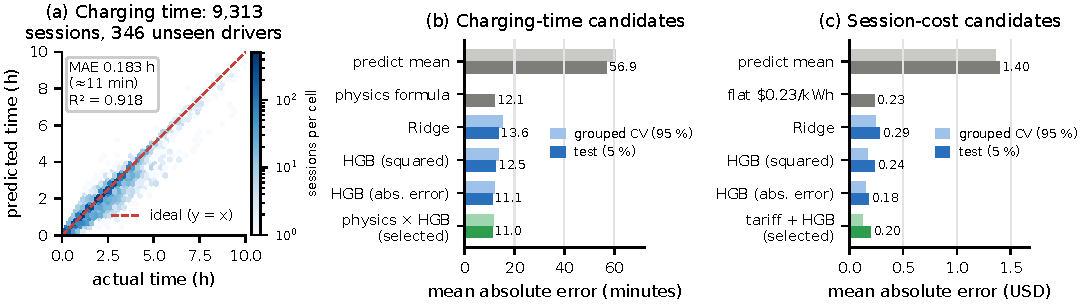
\includegraphics[width=\textwidth]{session_results.pdf}
  \caption{(a) Predicted vs.\ actual charging time for drivers never seen in training. (b, c) Every candidate model
  against the baselines; the model is chosen by grouped cross-validation (light bars), never by the test set.}
  \label{fig:session}
\end{figure}

\begin{figure}[!ht]
  \centering
  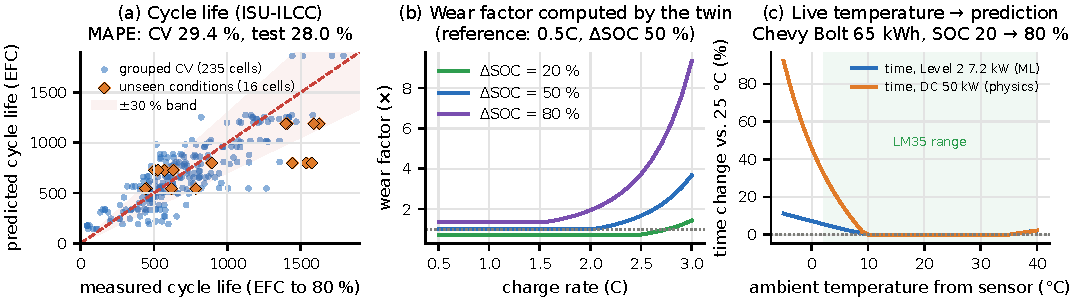
\includegraphics[width=\textwidth]{battery_sensor.pdf}
  \caption{(a) Cycle-life model on ISU-ILCC cells; cells tested under identical conditions already differ by
  $\approx$18\,\%, which bounds the achievable error. (b) Wear factor computed by the deployed twin from the life
  model. (c) The same request run through the deployed twin at different sensor temperatures.}
  \label{fig:battery}
\end{figure}

\textbf{Findings.} The hybrid charging-time model beats the physics formula by 9\,\% and the mean by 81\,\%. The cost
model learned a tariff of \textbf{\$0.2301/kWh} from the fees alone (published rate: \$0.23/kWh). Faster and deeper
charging raises wear (Fig.~\ref{fig:battery}b), and a cold sensor reading lengthens the charge
(Fig.~\ref{fig:battery}c): at 0\degC{} the Level~2 time rises by 7.2\,\%, the DC time by 45.8\,\% and grid energy by
about 7\,\% (examples in Table~\ref{tab:examples}).

\begin{table}[!ht]
\centering\footnotesize
\caption{Example outputs of the running twin (SOC 20 $\rightarrow$ 80\,\% unless stated, 25\degC{} unless stated).}
\label{tab:examples}
\begin{tabularx}{\textwidth}{@{}Y*{6}{r}@{}}
  \toprule
  \textbf{Request (vehicle, battery, age, charger)} & \textbf{Time} & \textbf{kWh} & \textbf{Cost \$} &
      \textbf{SOH \%} & \textbf{Wear} & \textbf{RUL EFC} \\
  \midrule
  Tesla Model 3, 75\,kWh, 3 y, DC 150\,kW      & 22\,min      & 45.8 & 21.97 & 94.6 & 1.10 & 1322 \\
  Tesla Model 3, 75\,kWh, 3 y, Level~2 11\,kW  & 4\,h 52\,min & 47.3 & 10.88 & 94.6 & 1.10 & 1322 \\
  Nissan Leaf, 40\,kWh, 5 y, Level~1           & 15\,h 16\,min& 25.7 &  5.91 & 91.0 & 1.10 &  996 \\
  Chevy Bolt, 65\,kWh, 4 y, Level~2 7.2\,kW    & 6\,h 18\,min & 40.2 &  9.25 & 92.8 & 1.10 & 1159 \\
  \quad same request, sensor reads 5\degC      & 6\,h 31\,min & 41.6 &  9.57 & 92.8 & 1.10 & 1159 \\
  Hyundai Kona, 64\,kWh, 2 y, DC 50\,kW, 10 $\rightarrow$ 90\,\% & 1\,h 05\,min & 53.1 & 25.47 & 96.4 & 1.34 & 1223 \\
  \bottomrule
\end{tabularx}
\end{table}

\textbf{System results.} The full three-laptop deployment worked end to end, and 151 automated tests pass (sensor 19,
ML worker and bridge 37, backend 62, frontend 33). With the real Arduino, a reading reached MQTT $\approx$0.5\,s after
its OPC~UA update, a ``live sensor'' request stored the board's temperature, and stopping the sensor raised a
\texttt{sensor\_offline} alert after 33\,s that cleared itself when readings resumed.

% =====================================================================
\section{AI/ML Details}
\subsection{Algorithms}
\begin{itemize}
  \item \textbf{Histogram gradient boosting} (scikit-learn~\cite{skl}): decision trees where each tree fits the errors
        of the previous ones (400 trees, learning rate 0.05, 63 leaves, $\geq$50 samples per leaf, L2 penalty 1.0),
        with absolute-error loss so that a few very long sessions do not dominate.
  \item \textbf{Hybrid physics + ML:} for time the trees learn the ratio $t_\mathrm{actual}/t_\mathrm{ideal}$ and the
        prediction is $t_\mathrm{ideal}\times$ ratio; for cost a learned \$/kWh tariff plus trees for the other fees.
        Both stay physically sensible outside the training range.
  \item \textbf{Ridge regression} with degree-2 polynomial features on $\log(\text{life})$ for battery cycle life,
        chosen for the lowest cross-validated percentage error and a smooth response. Also compared: linear Ridge,
        random forest, extra trees, Gaussian process and a ``predict the mean'' baseline.
\end{itemize}

\subsection{Training and testing process}
\begin{enumerate}
  \item Download, clean and build features (\texttt{prepare\_*.py}).
  \item Split 95/5 \textbf{by group}, never by random rows: by driver, by test condition (ISU) or by cell (NASA), so
        the test measures performance on new users and batteries.
  \item Choose the model by \textbf{grouped cross-validation} on the 95\,\% only (5 folds for sessions, 10 for ISU,
        leave-one-cell-out for NASA); the test set is used once, for reporting.
  \item Refit the chosen model; save it as \texttt{.joblib} with metadata (features, scores, split, date, version).
  \item Test the service: behaviour tests (``DC faster than Level~2'', ``cold is slower''), schema tests, ACN test.
\end{enumerate}

\subsection{How the ML model works inside the digital twin}
The trained models are not only used offline: they run on every request inside the live loop of the twin.
\begin{enumerate}
  \item \textbf{Real-time data in.} The LM35 reading travels Arduino $\rightarrow$ serial $\rightarrow$ OPC~UA
        $\rightarrow$ bridge $\rightarrow$ MQTT $\rightarrow$ backend every 5\,s. The backend stores it, flags jumps
        over 1\degC/s as \emph{suspect}, pushes it to the browser and raises an alert if readings stop for 30\,s.
  \item \textbf{Request.} An operator enters the vehicle, SOC window and charger. With source ``live sensor'' the
        backend inserts the newest sensor reading, refusing the request if the sensor is not live (a stale value is
        never used), then publishes it on MQTT with a 15\,s timeout.
  \item \textbf{Inference.} The ML worker (models loaded once at start-up) validates the message, drops duplicates,
        runs the physics model with the live temperature, then the ML models: time and cost for Level~1/2, and wear
        factor, wear and RUL from the life model. One prediction takes about 11\,ms.
  \item \textbf{Twin update.} Results return over MQTT, are stored in MongoDB with model versions and source labels,
        and are pushed to the dashboard. When a session is started on a bay, the \textbf{predicted duration and
        energy drive the 3D twin}: the bay turns blue and the car's SOC and energy rise on a clock running
        60$\times$ faster than real time (Fig.~\ref{fig:twin}).
\end{enumerate}
The ML thus makes the twin \emph{predictive}: it answers ``what happens if this car charges here now?'' from the live
temperature, behaviour learnt from 225{,}000 real sessions and ageing learnt from 251 cells.

\begin{figure}[!ht]
  \centering
  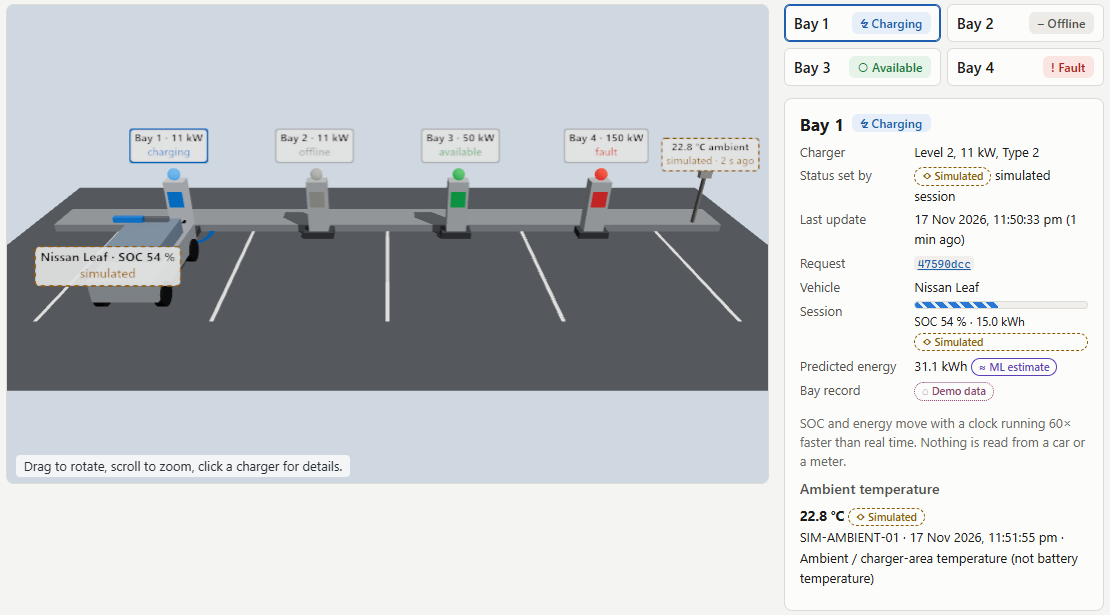
\includegraphics[width=0.56\textwidth]{twin_3d.png}
  \caption{3D station twin (Three.js): bay 1's session is driven by the ML-predicted duration and energy.}
  \label{fig:twin}
\end{figure}

% =====================================================================
\section{Limitations and Conclusion}
Battery outputs are estimates, not battery-management-system (BMS) readings: SOH comes from vehicle age, and wear and
RUL transfer the \emph{relative} effect of charge rate and depth from lab cells to an assumed 2{,}000-cycle pack. DC
predictions are physics-based (no public DC session data). Training data reach only 7\,kW, so faster Level~2 charging
is scaled from the physics time, with a warning. The LM35 measures air, not battery, temperature, and security suits
a lab LAN only. \textbf{Conclusion:} the project closes a complete digital-twin loop: a physical sensor feeds an
industrial protocol stack (OPC~UA, MQTT), and ML models validated on unseen users and cells run on every request and
drive a live 3D twin. Next steps are closed-loop charger scheduling and real charger and BMS data.

{\footnotesize
\begin{thebibliography}{9}\setlength{\itemsep}{0pt}
  \bibitem{pa} City of Palo Alto, ``Electric Vehicle Charging Station Usage (July 2011 -- Dec 2020),'' open data portal.
  \bibitem{acn} Z.\ J.\ Lee, T.\ Li, S.\ H.\ Low, ``ACN-Data: Analysis and Applications of an Open EV Charging
        Dataset,'' \emph{Proc.\ ACM e-Energy}, 2019.
  \bibitem{isu} T.\ Li, J.\ Liu, A.\ Thelen, C.\ Tischer, C.\ Hu, ``Predicting Battery Lifetime Under Varying Usage
        Conditions from Early Aging Data,'' arXiv:2307.08382, 2023.
  \bibitem{nasa} B.\ Saha, K.\ Goebel, ``Battery Data Set,'' NASA Prognostics Data Repository, NASA Ames, 2007.
  \bibitem{skl} F.\ Pedregosa \emph{et al.}, ``Scikit-learn: Machine Learning in Python,'' \emph{JMLR} 12, 2011.
\end{thebibliography}
}

\end{document}
